\section{Использование УОР-матриц}

Дана УОР-матрица $U$ ширины $k$, пусть $H$ --- абелева группа всех функций из $U \times [k]$ в циклическую группу $Cyc_m$ ($H$ является группой относительно поточечного сложения). Симметрическая группа $S_U$ действует на $H$ следующим образом:
\[
	\pi(h)(u,i)=h(\pi^{-1}(u),i)
\]
для $\pi \in S_U, \; h \in H, \; u \in U$ и $i \in [k]$. Интуитивно можно смотреть на элементы из $H$ как на таблицы того же размера что и $U$. Отличие в том, что в таблицах, соответствующих элементам из $H$, стоят элементы из $Cyc_m$, а не числа из $\left\{ 1,2,3 \right\}$. Эти таблицы можно складывать по правилам сложения обычных матриц. Действие $\pi \in S_U$ на $h \in H$ будет переставлять строки в соответствующей таблице.

Пусть $G$ --- полупрямое произведение $H \rtimes S_U$, определим подмножества $S_1, S_2, S_3$ так: $S_i$ состоит из всех произведений $h \pi$, где $\pi \in S_U$, и элемент $h \in H$ удовлетворяет условию:
\[
	h(u,j) \neq 0 \iff u_j=i
\]
для всех $u \in U$ и $j \in [k]$. Возвращаясь к аналогии с таблицами, у таблицы $h$ в данной позиции стоит ненулевой элемент тогда и только тогда, когда в соответствующей позиции  УОР-матрицы $U$ стоит $i$. На перестановку $\pi$ ограничения не налагаются.
\begin{figure}[H]
	\centering
    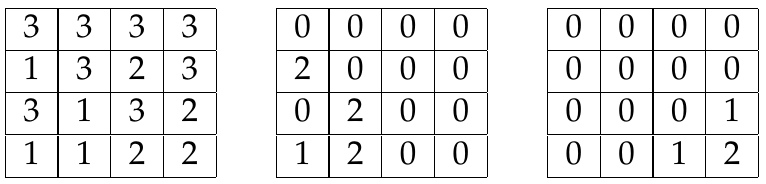
\includegraphics[width=0.5\textwidth]{figures/small_usp_and_group_elements}
	\caption{небольшая УОР-матрица и элементы группы $H$}
	\label{usp:fig3.6}
\end{figure}

На рисунке \ref{usp:fig3.6} показан пример небольшой УОР-матрицы $U$, справа от которой пара элементов из $H$, где $m=3$, и поэтому в них стоят числа из $\left\{ 0,1,2 \right\}$. Здесь элемент, стоящий в центре, будет содержаться в $S_1$, тогда как элемент справа не входит ни в одно из множеств $S_i$.

\begin{prop}\label{prop:05:3.5}
  Если $U$ --- УОР-матрица, то $S_1, S_2, S_3$ удовлетворяют свойству тройного произведения.
\end{prop}
\begin{proof}
  Рассмотрим тройное произведение
  \begin{equation} \label{eq:3.1}
  	h_1 \pi_1 \pi_1'^{-1} h_1'^{-1} h_2 \pi_2 \pi_2'^{-1} h_2'^{-1} h_3 \pi_3 \pi_3'^{-1} h_3'^{-1} = 1, \text{ где } h_i \pi_i, h_i' \pi_i' \in S_i.
  \end{equation}
  
  Если привести это уравнение по всем правилам, действующим в полупрямых произведениях, получим
  \[
  	(h_1 + \pi_1 \pi_1'^{-1} \cdot (h_1'^{-1}h_2) + \pi_1 \pi_1'^{-1} \pi_2 \pi_2'^{-1} \cdot (h_2'^{-1}h_3) + \pi_1 \pi_1'^{-1} \pi_2 \pi_2'^{-1} \pi_3 \pi_3'^{-1} \cdot h_3'^{-1}) \pi_1 \pi_1'^{-1} \pi_2 \pi_2'^{-1} \pi_3 \pi_3'^{-1} = 1,
  \]
  где всё, что стоит в скобках является элементом из $H$, <<$\cdot$>> как обычно обозначает действие. Стоит заметить, что так как $H$ абелева, то операция в ней будет иметь аддитивную форму, то есть все $h_i'^{-1}$ впоследствии будут преобразованы в $-h_i'$.
  
  Чтобы \eqref{eq:3.1} выполнялось должно быть 
  \begin{equation} \label{eq:3.2}
  	\pi_1 \pi_1'^{-1} \pi_2 \pi_2'^{-1} \pi_3 \pi_3'^{-1} = 1.
  \end{equation}
  Зададим $\pi = \pi_1 \pi_1'^{-1}$ и $\rho = \pi_1 \pi_1'^{-1} \pi_2 \pi_2'^{-1}$. Тогда для того, чтобы \eqref{eq:3.1} было верно в группе $H$ должно выполняться условие:
  \begin{equation} \label{eq:3.3}
  	h_1 - h_3' + \pi (h_2 - h_1') + \rho (h_3 - h_2') = 0.
  \end{equation}
  
  Обратите внимание, что
  \begin{align*}
  	(h_1 - h_3')(u,j) & \neq 0  \iff  u_j \in \left\{ 1,3 \right\}\\
  	\pi(h_2 - h_1')(u,j) & \neq 0 \iff  (\pi^{-1}(u))_j \in \left\{ 2,1 \right\}\\
  	\rho(h_3 - h_2')(u,j) & \neq 0 \iff  (\rho^{-1}(u))_j \in \left\{ 3,2 \right\}.
  \end{align*}
  
  По определению УОР-матрицы либо $\pi=\rho=1$, либо существуют $u$ и $j$ такие, что в точности одно из этих трёх условий выполняется, но в этом случае \eqref{eq:3.3} не может быть верным.
  
  Теперь тоже самое, но подробнее. Рассмотрим следующую тройку перестановок $\rho^{-1}, 1, \pi^{-1} \in S_U$, из определения УОР-матрицы получим, что либо $\rho^{-1}= 1= \pi^{-1}$ либо $\exists u \in U, j \in [k]$ такие, что в точности 2 из 3 равенств $(\rho^{-1}(u))_j=1, u_j=2, (\pi^{-1}(u))_j=3$ верны. Пусть не выполняется первое равенство, тогда:
  \begin{align*}
  		(\rho^{-1}(u))_j \in \left\{ 2,3 \right\} & \implies \rho(h_3-h_2')(u,j) \neq 0\\
  		u_j = 2 & \implies (h_1 - h_3')(u,j) = 0\\
  		(\pi^{-1}(u))_j=3 & \implies \pi(h_2 - h_1')(u,j) = 0.
  \end{align*}
  
  Откуда следует, что \eqref{eq:3.3} не может выполняться, так как одно из слагаемых не равно нулю. Аналогично рассматриваются случаи, когда $u_j \neq 2$ и $(\pi^{-1}(u))_j \neq 3$.
  
  Таким образом, $\pi=\rho=1$, что вместе с \eqref{eq:3.2} означает $\pi_i = \pi_i'$ для всех $i$. Тогда имеем $h_1+h_2+h_3=h_1'+h_2'+h_3'$, откуда получаем $h_i'=h_i$ для всех $i$ потому, что только у $h_i$ и $h_i'$ в таблицах ненулевые элементы стоят в одних и тех же позициях. В итоге свойство тройного произведения выполняется.
\end{proof}

\begin{corollary}\label{cor:05:3.6}
  Если $U$ --- УОР-матрица ширины $k$ и $m \geq 3$, тогда 
  \[
  	\omega \leq \frac{3 \ln m}{\ln(m-1)} - \frac{3 \ln |U|!}{|U| k \ln(m-1)}
  \]
  В частности, если УОР-ёмкость равна $C$, тогда
  \[
  	\omega \leq \frac{3(\ln m - \ln C)}{\ln(m-1)}.
  \]
\end{corollary}
\begin{proof}
  Если $G$ реализует $\left\langle |S_1|,|S_2|,|S_3| \right\rangle$, то из следствия \ref{cor:05:1.9} и того, что $|G:H|=|U|!$ является наибольшей степенью неприводимого характера $G$, получим
  \begin{equation}\label{eq:s}
  	(|S_1||S_2||S_3|)^{\omega/3} \leq (|U|!)^{\omega-2}|G|.
  \end{equation}
  Мощность множества
  \[
  	|S_i|=(m-1)^{\text{количество $i$ в $U$}}\cdot |U|!.
  \]
  Итого
  \[
  	|S_1||S_2||S_3| = (m-1)^{|U|k}(|U|!)^3.
  \]
  Отмечу, что $|H|=m^{|U|k}$. Следовательно $|G|=m^{|U|k}|U|!$. Подставив в \eqref{eq:s} посчитанные значения получим:
  \begin{align*}
  	((m-1)^{|U|k}(|U|!)^3)^{\omega/3} & \leq (|U|!)^{\omega-2}m^{|U|k}|U|!\\
  	(m-1)^{\frac{|U|k}{3} \omega} (|U|!)^\omega & \leq \frac{m^{|U|k}}{|U|!}(|U|!)^\omega\\
  	\omega \frac{|U|k}{3} \ln (m-1) & \leq \ln \frac{m^{|U|k}}{|U|!}\\
  	\omega & \leq 3 \frac{|U|k \ln m - \ln |U|!}{|U|k \ln(m-1)} = \frac{3 \ln m}{\ln (m-1)} - \frac{3 \ln |U|!}{|U|k \ln(m-1)}.
  \end{align*}
  Из формулы Стирлинга легко получить, что
  \[
  	\ln n! = \ln \frac{n^n}{e^n} \sqrt{2 \pi n} (1 + o(1)) = n \ln n (1 + o(1)).
  \]
  \begin{question}
    Как выводятся друг из друга различные формы формулы Стирлинга?
    \begin{align*}
      \ln n! & = n \ln n - n + O(\ln(n))\\
      \ln n! & = n \ln n (1 + o(1)) \overset{?}{=} n \ln (n (1 + o(1)))
    \end{align*}
  \end{question}
  По определению УОР-ёмкости $C$ найдутся такие $U$, что $|U|=(C - o(1))^k$.
  \[
  	\frac{3 \ln |U|!}{|U|k \ln(m-1)} = \frac{3 \cancel{|U|} \ln |U| (1+o(1))}{\cancel{|U|}k \ln (m-1)} = \frac{3 \cancel{k} \ln (C - o(1))}{\cancel{k} \ln (m-1)}.
  \]
  \begin{question}
    Правильно ли я здесь обращаюсь с $o(1)$?
  \end{question}
  В итоге
  \[
  	\omega \leq \frac{3 \ln m}{\ln (m-1)} - \frac{3 \ln C}{\ln (m-1)} = \frac{3 (\ln m - \ln C)}{\ln (m-1)}. \qedhere
  \]
\end{proof}

С помощью утверждения \ref{prop:05:3.1} можно получить оценку $\omega < 2.67$ при $m=9$. В следующем разделе будет показано, что УОР-ёмкость по меньшей мере равна $2^{2/3}$, и поэтому $\omega < 2.48$, что является наилучшей известной оценкой, полученной при помощи УОР-матриц.

Если гипотеза \ref{conj:05:3.4} верна, то следствие \ref{cor:05:3.6} даст оценку $\omega = 2$ при $m=3$.



